
\section{Web layout}

Web page source code is written in HTML,
  which is a tree-structured markup language
  containing text and elements that wrap it.
The web browser's parsed representation of this tree
  is called the DOM tree.
To draw the page to the screen,
  the browser applies a sequence of transformations---%
  rendering phases---%
  to this DOM tree: matching, styling, layout, paint, and so on.
The focus of this paper, the layout phase,
  applies to an intermediate tree structure
  called a ``layout tree'',
  whose shape largely matches the DOM tree,
  though with some deviations.
The layout phase reads properties from layout tree nodes
  (which reflect HTML attributes, CSS properties, and other data)
  and computes layout fields like width and height for those nodes.
Later phases like paint then read those layout fields
  and use them to draw the page to the screen.
In memory,
  the layout tree is stored as a pointer tree,
  with the children stores as a doubly linked list.
This is necessary for fast insertions and deletions,
  but also means that layout nodes are
  often spread throughout memory,
  with every access generating a cache miss.


\begin{figure}
\scalebox{0.7}{
\begin{forest}
  [body 
    [header [a] [div [nav [a] [a] [a] [a] [a]] [nav [a]]]]
    [div 
      [ol 
        [li 
          [div 
            [div [a] [div]] 
            [div 
              [span [a]] 
              [span [a] [a]]
              [a]
              [div 
                [a [img]] 
                [span]
                [a]
                [span]
                [span]
                [span [input] [label [div [a] [a] [a]]]] 
                [span [span] [a]]]]]]
        [a [span]]]
    [div]
    [ol
      [li
        [div
          [form
            [input]
            [input]
            [input
              [div
                [textarea
                  [p]
                  [div
                    [input] [button] [div]]]]
              [p]]]]]
      [li]]]
    [footer [a] [a] [a] [a]]
    [span]]
\end{forest}
}
\centering
\caption{A dom tree representation
  of a page on \texttt{lobste.rs},
  an online forum / news aggregator,
  with just a single link and no comments.
Text nodes are not shown.
The page nonetheless contains 69 elements,
  with the maximum width of 7 and maximum depth of 10;
  in other words, the page is highly imabalanced.
Among the links (\texttt{<a>} elements),
  the spine+1 can contain as many as 30 elements, half the complete tree,
  due to the unbalanced tree.
  \todo{Compress in the vertical dimension}}
% https://lobste.rs/s/7ixd88/c_complexity_compiler_bugs
\label{fig:dom-tree-raw}
\end{figure}

\subsection{The Layout Phase}

Computing layout fields is a recursive process
  because each node's layout depends on the layout of its neighbors.
For example, the height of a node is (typically)
  the sum of the heights of all its children,
  while a node's $x$ position depends on the $x$ position
  of its previous sibling, plus that previous sibling's width.%
\footnote{
  In reality, these rules are quite a bit more complex,
    with various exceptions to the simplified sketch given here.}
Moreover, visible properties like width and height
  in turn depend on intermediate properties such as intrinsic size,
  current line width/height, and more obscure properties
  like the sum of its siblings' \texttt{flex-grow} values.
A complete layout pass must visit each node multiple times,
  in a well-defined order,
  in order to compute each field on each node
  before any others that depend on it.

\begin{figure}
\begin{verbatim}
def layout_simple(self): # real layout much more complex
  for c in self.children:
    layout_simple(c)
  self.height <-
    if has_path(last) then last.height_acc 
    else self.attribute[height]
  self.height_acc <-
    if has_path(prev) then prev.height_acc + self.height 
    else 0
\end{verbatim}
\caption{A layout algorithm that compute width of each dom node. The above program is a tree traversal: it walk down the tree then walk up the tree, computing values for each node during the walk.
}
\label{fig:layout-simple}
\end{figure}

\iffalse
\begin{figure}
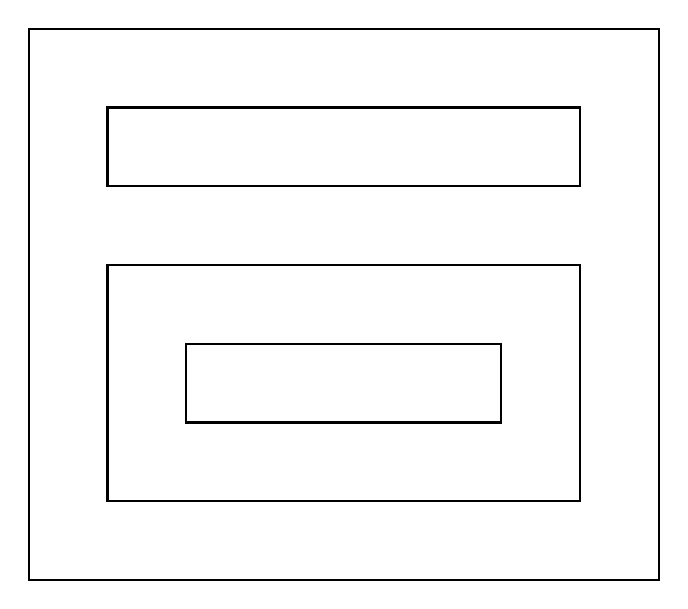
\begin{tikzpicture}
\draw[black, thick] (0,7) rectangle (8,0);
\draw[black, thick] (1,6) rectangle (7,5);
\draw[black, thick] (1,4) rectangle (7,1);
\draw[black, thick] (2,3) rectangle (6,2);
\end{tikzpicture}
\caption{The HTML document is laid-out into multiple boxes, forming a tree.}
\end{figure}
\fi

\begin{figure}
\centering
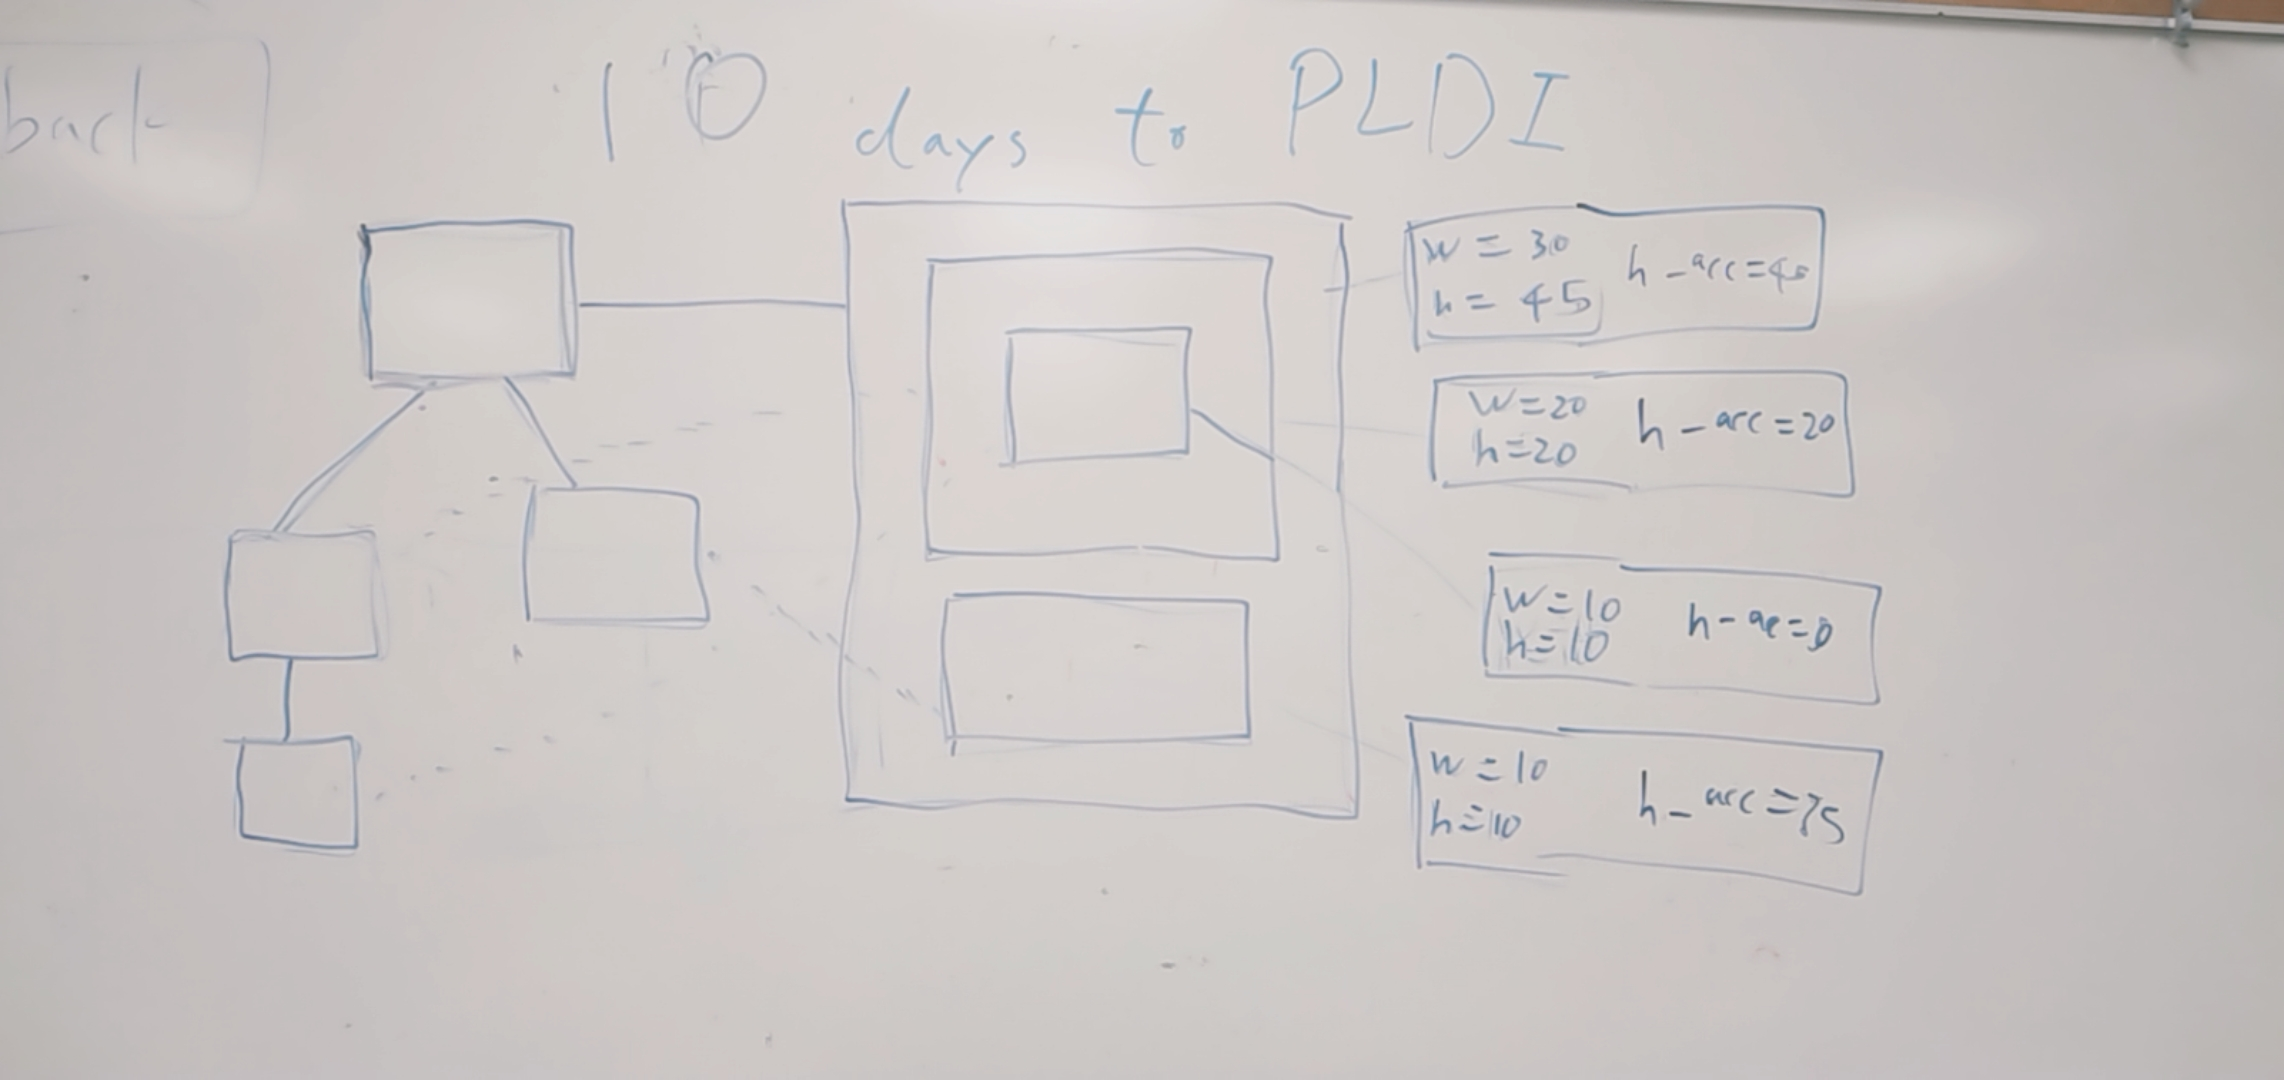
\includegraphics[scale=0.15]{layout.jpg}
\caption{A tree, its property, and the box model}
\end{figure}

We remark on a couple of key properties of layout
  that influence our approach:
\begin{enumerate}
    \item{Bounded work}: a fixed, bounded amount of work is performed per node. There are no data-dependent loops, recursions, or data structures except over the layout tree itself.
    \item{Immutable shape}: the layout tree itself is not modified during layout; only the computed fields on each node are. Moreover, these computed fields are only written once (per frame) and then become read-only (for that frame).
    \item{Static control flow}: the fields are computed in a fixed order dependent only on the layout tree shape, not the values of other computed fields.
    \item{Local data flow}: to compute a particular node's fields, only that node's neighbors in the layout tree and their fields are accessed.
\end{enumerate}
In other words, layout can be expressed in the DSL
  shown in Figure~\ref{fig:dsl}.

In this DSL, a layout is defined by a set of passes
  $\text{Pass}_n$ performed in a certain order (the schedule).
Each pass performs a recursive, in-order traversal of the tree,
  computing some fields pre-order and some fields post-order.
Computing a field just requires
  a simple assignment $\mathsf{self}.V \gets T$,
  where $V$ is a computed field on the current node $\mathsf{self}$
  and $T$ is an expression that can refer to
  other fields on $\mathsf{self}$ and its neighbors
  $\mathsf{parent}$, $\mathsf{prev}$, $\mathsf{next}$,
  $\mathsf{first}$ (child), and $\mathsf{last}$ (child).
Computations can also refer to HTML attributes or CSS properties
  of the DOM node corresponding to the current layout node
  using $\mathsf{attribute}[x]$ or $\mathsf{property}[x]$.%
\footnote{
    We use two different namespaces
    for HTML attributes and CSS properties
    because some names, like \texttt{height},
    appear in both sets.
    There's a special property for the tag name.
    The exact details differ between browsers
    but do not affect spineless traversal,
    so we ignore the distinctions here.
}
Expressions can also use conditionals
  to test whether a given neighbor exists ($\mathsf{N?}$).
The DSL is more flexible than it may at first appear:
  for example, if a node wants to access a field on its grandparent,
  instead of accessing $\mathsf{parent}.\mathsf{parent}.\mathsf{x}$,
  each node could define a $\mathsf{parent\_x}$ field which copies
  its parent's $x$ value,
  and then access $\mathsf{parent}.\mathsf{parent\_x}$.
In any case, prior work in similar DSLs%
  ~\cite{meyerovich-1, meyerovich-2, cassius-1,
  cassius-2, cassius-3, yufeng-1, yufeng-2}
  has already shown that layout features
  like the CSS box model, \texttt{display: none},
  absolute positioning, flexible box layout,
  and line breaking are expressible in such a language.

A key property of a layout $L$
  is the order in which it computes
  different fields on different nodes in the tree.
Specifically, let the \emph{trace} of a layout on a tree $T$
  be sequence of $(n, v)$ pairs
  where $n$ is a node in $T$ and $v$ is a field name in $L$.
Because our DSL only performs in-order traversals,
  the trace is structurally related to the tree shape:
  local changes to the tree (node insertions or deletions)
  imply local change to the trace (subtrace insertion or deletion).
This structural relation means
  that the ordering of any two $(n, v)$ pairs is fixed:
  if $(n, v)$ appears before $(n', v')$,
  this appear-before relationship
  will be maintained even as new nodes are added or removed.% 
\footnote{
  We assume here that
    only brand-new nodes, not previously-removed ones,
    are inserted into the tree.
  To our knowledge, this assumption is true
    of all major web rendering engines.
}

In the remainder of this paper,
  we will assume a correct implementation
  of web page layout exists in this DSL,
  with correctness meaning both the correct set of rules
  and also a correct schedule for computing them
  while preserving dependencies.
Our own implementation (Section~\ref{sec:layout-impl})
  implements a subset of widely-used web layout features;
  however, spineless traversal is applicable
  to any layout expressed in this DSL,
  and we do not focus on the details
  of the rules or schedule further.
Notably, our DSL enforces
  the key properties of layout described above:
  there is no functionality to mutate the tree shape
  or to reorder control flow according to field values.
There are also no loops or data structures,
  and the only field access allowed is to a node's neighbors.

\begin{figure}

\begin{align*}
\text{Layout} &\coloneq  \{\:
  \mathsf{rules}: \text{Rule}^+,
  \mathsf{schedule}: \text{Pass}_n^+
\:\} \\
\text{Rule} &\coloneq
  \mathbf{def}\:\text{Pass}_n()\:\{\:
    A^+;\:
    \mathsf{children}.\mathsf{forEach}(\text{Pass}_n);\:
    A^+;\:
  \} \\
A \in \text{Assignment} &\coloneq
  \text{self}.V \leftarrow T \\[4pt]
T \in \text{Term} &\coloneq
  \text{if}\ T\ \text{then}\ T\ \text{else}\ T \mid
  F(T^+) \mid
  N? \mid
  N.V \mid
  \mathsf{attribute}[V] \mid
  \mathsf{property}[V] \\
N \in \text{Neighbor} &\coloneq
  \mathsf{self} \mid \mathsf{prev} \mid
  \mathsf{next} \mid \mathsf{parent} \mid
  \mathsf{first} \mid \mathsf{last} \\[4pt]
V \in \text{Variable} &\coloneq \text{unique symbols} \quad\quad
F \in \text{Function} \coloneq \text{primitive functions}
\end{align*}
\caption{
  A minimal DSL for defining web layout
    as a set (\textsf{rules}) of passes
    performed in a specific order (\textsf{schedule}).
  The syntax $P^+$ represents a sequence of non-terminal $P$.
  Passes are in-order traversals of the layout tree
    performing a sequence of assignments to local fields
    while accessing fields of the current node or its neighbors.
}
\label{fig:dsl}
\end{figure}


\subsection{Incremental layout}

Layout needs to be performed any time
  a user interaction or JavaScript code
  modifies the DOM tree,
  typically in response to a user interaction like
  clicks, hovers, drags, animations, or typing.
The DOM tree modification
  can change the value of an HTML attribute or CSS property
  (as happens when the user selects a drop-down item
  or types into a text box)
  or it can insert and delete nodes in the DOM
  (as might happen when a page is loaded or new content
  is inserted from the network),
  but most of these modifications,
  and especially the most latency-critical,
  like hovers, drags, animations, and text editing,
  modify only a small portion of the DOM tree at a time
In either case,
  once the DOM node changes,
  the layout tree must change as well.
If DOM nodes are added or removed,
  layout nodes typically must be as well;
  layout nodes can also be removed
  by modifying some HTML attribute (like \texttt{hidden})
  or CSS properties (like \texttt{display: none}).
Then, whether or not DOM nodes are added or removed,
  the computed value of various layout fields
  may change and need to be recomputed.

In order to achieve this,
  each layout node maintains a \textit{dirty} bit for each field,
  which defines whether that field value needs to be recomputed.%
\footnote{In a real browser, often one boolean bit
  summarizes whether any in a set of fields need to be recomputed,
  but we describe a bit per field here for simplicity.}
The dirty bit is set when a layout node is added to the tree,
  and is cleared when its associated field is computed.
A field is also dirtied when a value it depends on changes.
For example, in the simple layout of Figure~\ref{fig:layout-simple},
  when a node's \texttt{height} attribute is changed,
  its \texttt{height} field is marked dirty.
Then, when that \texttt{height} field is recomputed,
  its \texttt{height\_acc} field can in turn be marked dirty.
When the \texttt{height\_acc} field is recomputed,
  its next sibling's \texttt{height\_acc} field is then marked dirty.
Alternatively, if a node is deleted,
  the \texttt{height} of its parent
  (if it was the last child)
  and the \texttt{height\_acc} of its next sibling
  must be marked dirty.

However, recomputing a field does not mark any dependent fields
  if the newly-computed value matches the previous value.
This optimization is critical:
  it means that many changes affect only a
  small fraction of the layout tree,
  since their effects are localized to a subset of it.
For example, you might imagine that typing into a multi-line text box
  can move around the text within the text box
  but, if the text box has a fixed height,
  won't affect the size or position of anything outside it.
In other words, fields are marked dirty when
  HTML attributes or CSS properties change,
  or when nodes are added and removed from the DOM;
  then these dirty bits propagate through the layout tree
  until all affected nodes are marked and recomputed.%
\footnote{
  As described this is a flow-insensitive dependency analysis;
    it is possible to do a finer-grained flow-sensitive analysis instead.
  This design decision is orthogonal to the algorithms presented in this paper.
}

Importantly, dirty bit propagation code
  can be synthesized from the layout algorithm.
To do so, one analyzes every assignment $\mathsf{self}.V \gets T$
  in the layout program.
For each field access $N.U$ in the expression $T$,
  we know that $\mathsf{self}.V$ depends on $N.U$,
  meaning that any changes to $\mathsf{self}.U$
  must mark $N^{-1}.V$ as dirty,
  where $N^{-1}$ is the inverse of the relation $N$;
  flipping \textsf{next} and \textsf{previous},
  mapping \textsf{first} and \textsf{last} to \textsf{parent},
  and mapping \textsf{parent} to all children.
Note that, if the original algorithm respects the dependency order,
  then a field is only computed after all fields that it depends on.
This in turn means that, after a field is computed,
  it can no longer be marked dirty.
This guarantees termination:
  computing a field clears its dirty bit, so by the end of an incremental layout
  every field is clean.

Insertion and deletion require particular care
  in propagating dirty bits.
An inserted node has all of its new fields marked dirty;
  likewise, deleting a node marks all dependants of its fields.
Inserting or deleting nodes can also change
  $\mathsf{N?}$ expressions;
  any fields that use such expressions must then
  also be marked dirty.%
\footnote{Once again,
  this could use a flow-sensitive analysis or a simpler
  flow-insensitive one.
The invalidation challenges are similar in either case.}
Importantly, an entire subtree can be inserted or deleted at once;
  this is quite common in real-world web pages
  where pop-ups or menus can appear as a result of a hover or click.
Since all data accesses in our model are local,
  only the root of the subtree actually needs to be considered,
  meaning that deleting or inserting a subtree takes constant time,
  regardless of the size of the subtree.

\subsection{Recomputation}
With the dirty bit marking algorithm mentioned above, 
  the problem of incremental layout is now reduced to 
  finding all dirtied fields, and recomputing them, 
  in the dependency order.

A naive incremental implementation can recursively traverse 
  the tree as if rerunning from scratch, 
  but only re-assign value to the dirtied node. 
This trivial invalidation algorithm nonetheless
  respects the dependency order and clears all dirtied fields.
It also recomputes only dirtied fields,
  performing a minimal number of recomputations.
However, since it traverses the entire tree,
  in incurs just as many cache misses as a non-incremental layout
  and therefore does not lead to a significant speed-up.
Driven by this observation, we can immediately classify
  accessed nodes into two types: the dirtied nodes,
  which have fields dirtied and must be accessed to
  recompute them, and the auxiliary nodes, 
  which does not have fields dirtied, but are nonetheless 
  accessed in order to find and reach the dirtied node.
The number of dirtied nodes is set by
  the dependency structure of web layout,
  but the number of auxiliary nodes can be reduced
  through better algorithms for finding dirtied nodes.

\subsection{Double Dirty Bit}
The SOTA algorithm,
  which we dub the Double Dirty Bit algorithm,
  achieves this by adding a second dirty bit
  per pass, which indicates whether
  any field assigned during pass
  is dirty in the \emph{subtree} rooted at a node.
This summary bit is initially off, and when a node is marked,
  the summary bit is turned on.
Since the summary bit is recursive over the subtree,
  setting a summary bit must also set the parent's summary bit,
  stopping at the root node
  or at a node with the summary bit already on.

\begin{figure}
\begin{minipage}[t]{0.4\linewidth}
\scriptsize
\begin{verbatim}
def find_dirty_nodes(self):
    if self.dirty:
        yield self
    if self.summary_bit:
        # Access spine + 1
        for child in self.children:
            find_dirty_nodes(child)
\end{verbatim}
\end{minipage}\hfill%
\begin{minipage}[t]{0.6\linewidth}
\caption{Finding the dirty nodes in a tree.}
\label{fig:find-dirty-nodes}
\end{minipage}
\end{figure}

The summary bit allows layout to skip recursing into a subtree
  when the summary bit is off.
An example implementation, conceived as an iterator
  that yields dirty nodes,
  is shown in Figure~\ref{fig:find-dirty-bits}.
The Double Dirty Bit algorithm
  greatly reduces the number of nodes accessed,
  improving performance,
  and is considered the state of the art
  for layout invalidation~\cite{tali-garseil,wbe}.

However, the Double Dirty Bit algorithm
  nonetheless accesses a number of auxiliary nodes.
To reach any dirty node,
  the Double Dirty Bit traversal must
  must traverse the path from the root of the tree
  to the dirtied node---the ``spine'' of that node.
Moreover, each node along that spine
  will have its summary bit set,
  meaning that the Double Dirty Bit algorithm will recurse
  into that node's children.
In other words,
  the Double Dirty Bit algorithm has, as its auxiliary nodes,
  both the spine of each dirtied node,
  and also all children of that spine.
Since web layout trees have both very wide and very deep nodes,
  this can be a very large set of auxiliary nodes.
For example, the \texttt{lobste.rs} web page
  shown in Figure~\ref{fig:dom-tree-raw}
  has an \texttt{<input>} element at depth 8,
  which represents a dropdown that a user might interact with.
An interaction like opening and closing the dropdown
  will affect only a few elements
  (likely seven:
    the \texttt{<input>},
    its sibling \texttt{<label>},
    and its parent \texttt{<span>}),
  but its spine contains eight nodes
  and adding the children of the spine nodes
  brings the total number of auxiliary nodes to 22.
If (oversimplifying) cache misses are the only cost,
  Double Dirty Bit would have then have
  $22 / 7 \approx 3\times$ overhead for this interaction,
  unnecessarily increasing latency.

Unsurprisingly, these auxiliary nodes
  are a significant source of latency,
  affecting both browser and web developers.
Google Chrome's Lighthouse performance monitoring tool~\cite{lighthouse},
  for example, warns if tree depth or fanout is high.
This implicitly means that achieving the expected performance,
  especially on a highly-interactive web application
  such as Figma, VS Code, Office 365, or Photoshop,
  may require changing the global shape of the layout tree.
Naturally, an invalidation algorithm that simply
  did not require so many auxiliary nodes
  would be a superior solution.

\begin{figure}
\scalebox{0.7}{
\begin{forest}
  [body 
    [header [a] [div [nav [a] [a] [a] [a] [a]] [nav [a]]]]
    [div 
      [ol 
        [li 
          [div 
            [div [a] [div]] 
            [div 
              [span [a]] 
              [span [a] [a]]
              [a]
              [div 
                [a [img]] 
                [span]
                [a]
                [span]
                [span]
                [span [input] [label [div [a,color=blue] [a, color=green, for ancestors={color=red, for siblings={color=blue}}, name=CurrentDirtied] [a, color=orange, name=NextDirtied]]]]
                {\draw[->,dotted] (CurrentDirtied)--(NextDirtied);}
                [span [span] [a]]]]]]
        [a [span]]]
    [div]
    [ol
      [li
        [div
          [form
            [input, color=blue]
            [input, color=yellow, for ancestors={color=red, for siblings={color=blue}}]
            [input, color=blue,
              [div
                [textarea
                  [p]
                  [div
                    [input] [button] [div]]]]
              [p]]]]]
      [li]]]
    [footer [a] [a] [a] [a]]
    [span]]
\end{forest}
}
\centering
\caption{The Double Dirty Bit algorithm in action. The green "a" is the dirtied node, with the spine marked red, and the siblings of the spine marked blue, forming the spine+1. We assume the green "a" dirtied its next sibling, the orange "a". Note that the subsequent marking only dirty nodes on the spine+1, or their children, so maintaining summary bits and finding subsequent dirty node is quick. Other node (in this case, the yellow 'input' element) might also be dirtied, and the spine is reused.}
% https://lobste.rs/s/7ixd88/c_complexity_compiler_bugs
\label{fig:dom-tree-db}
\end{figure}